\documentclass[utf8]{beamer}

\usepackage{graphicx}
\usepackage{epstopdf}

\mode<presentation>

\begin{document}

\title{QACG}

\begin{frame}

\titlepage

\end{frame}

\begin{frame}
  \frametitle{Controlled Addition} 
  \begin{figure} 
    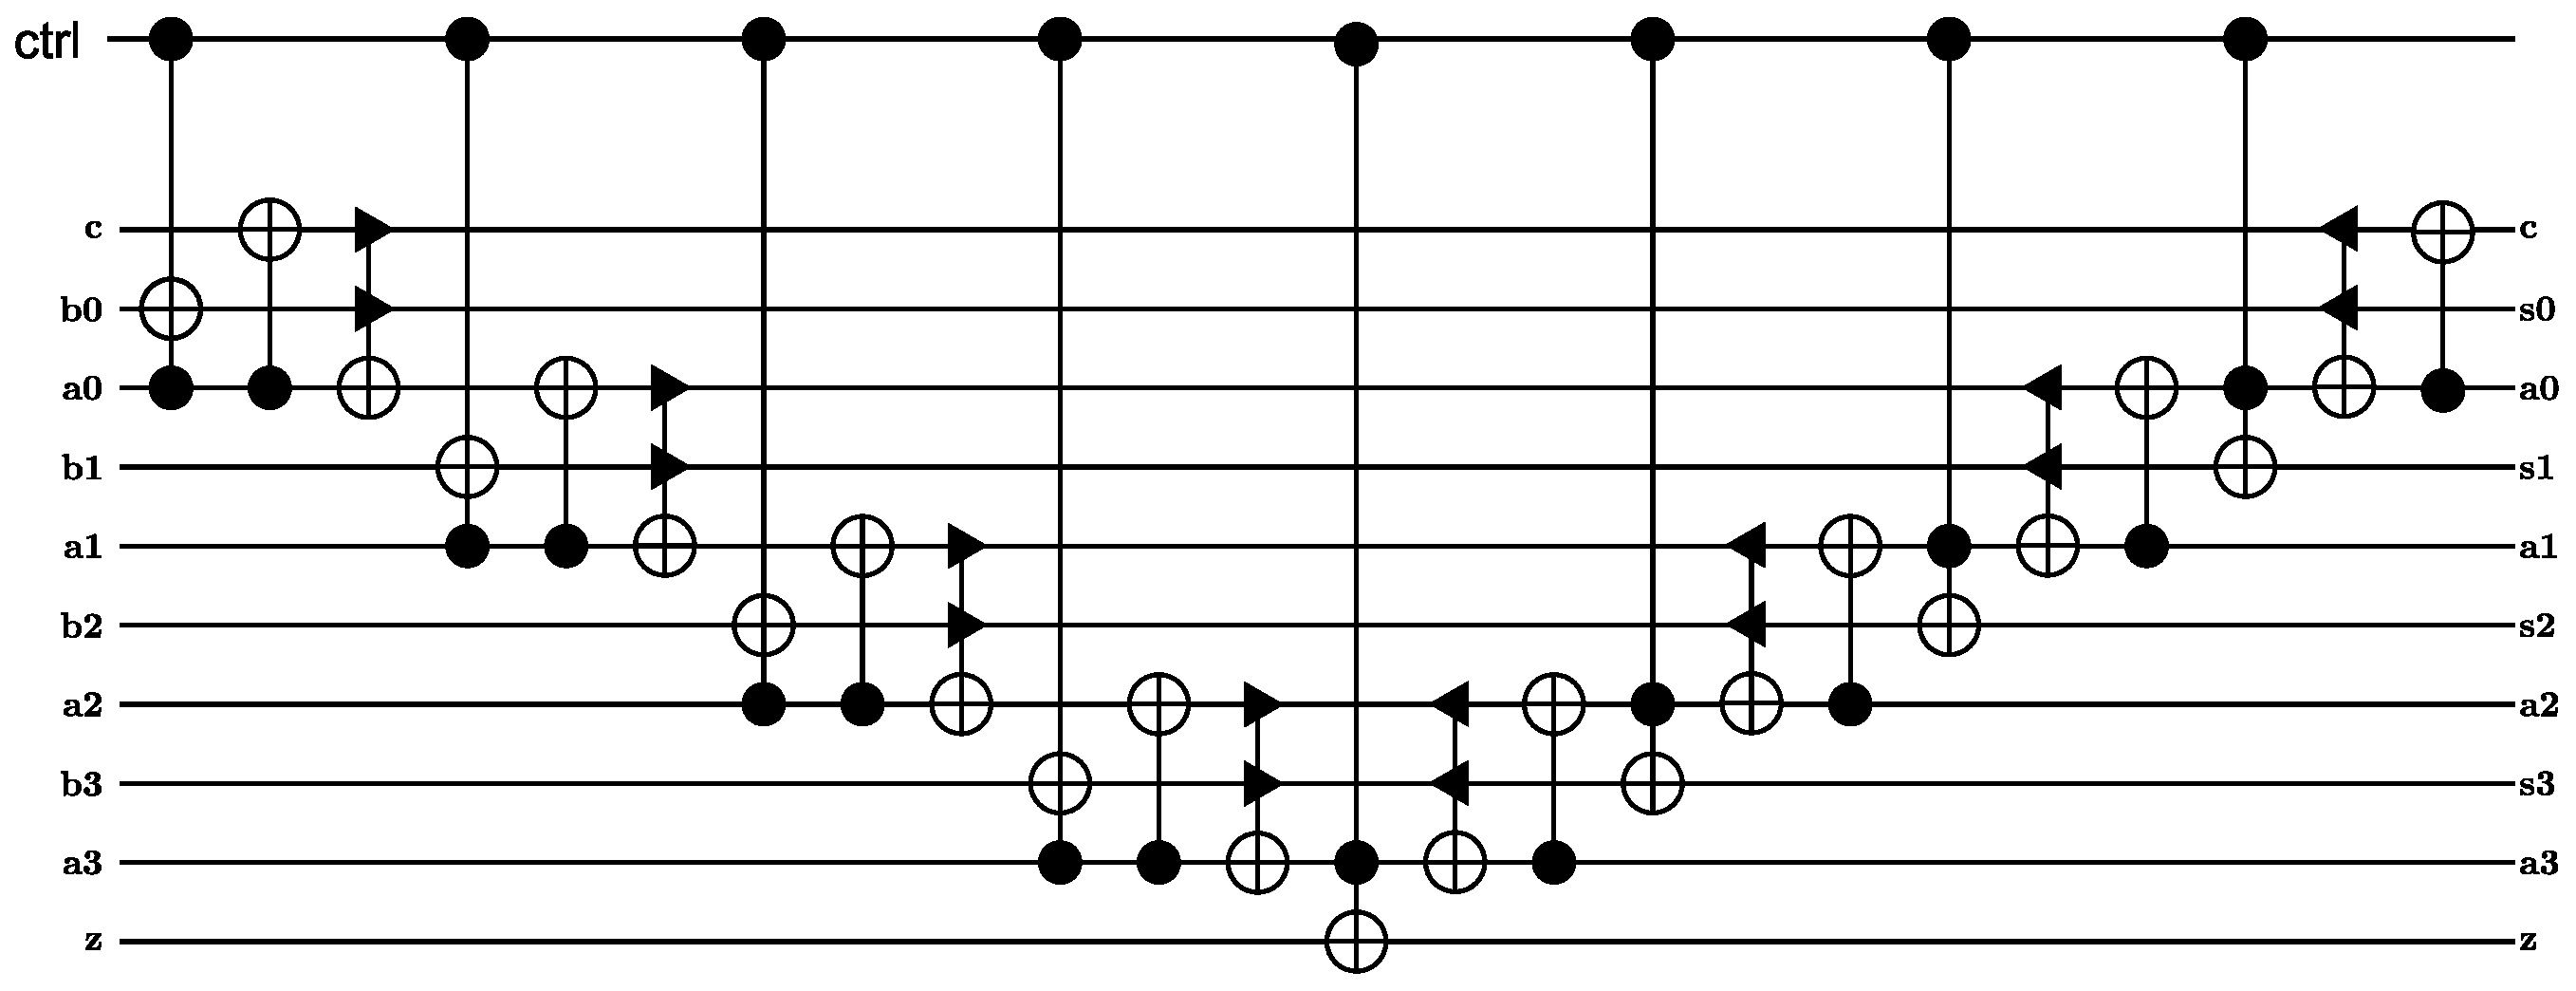
\includegraphics[width=\linewidth]{diagrams/4BitRippleAdderCtrl}
  \end{figure}
  Controlled version of the Cuccaro adder with the Selinger ``directional'' Toffoli optimization.
\end{frame}

\begin{frame}
  \frametitle{Multiplication}
  \begin{columns}
    \begin{column}{5cm}
      \begin{itemize}
        \item Shift and add (controlled addition)
        \item Tree based 
        \item Karatsuba
      \end{itemize}
    \end{column}
    \begin{column}{5cm}
      \begin{figure} 
        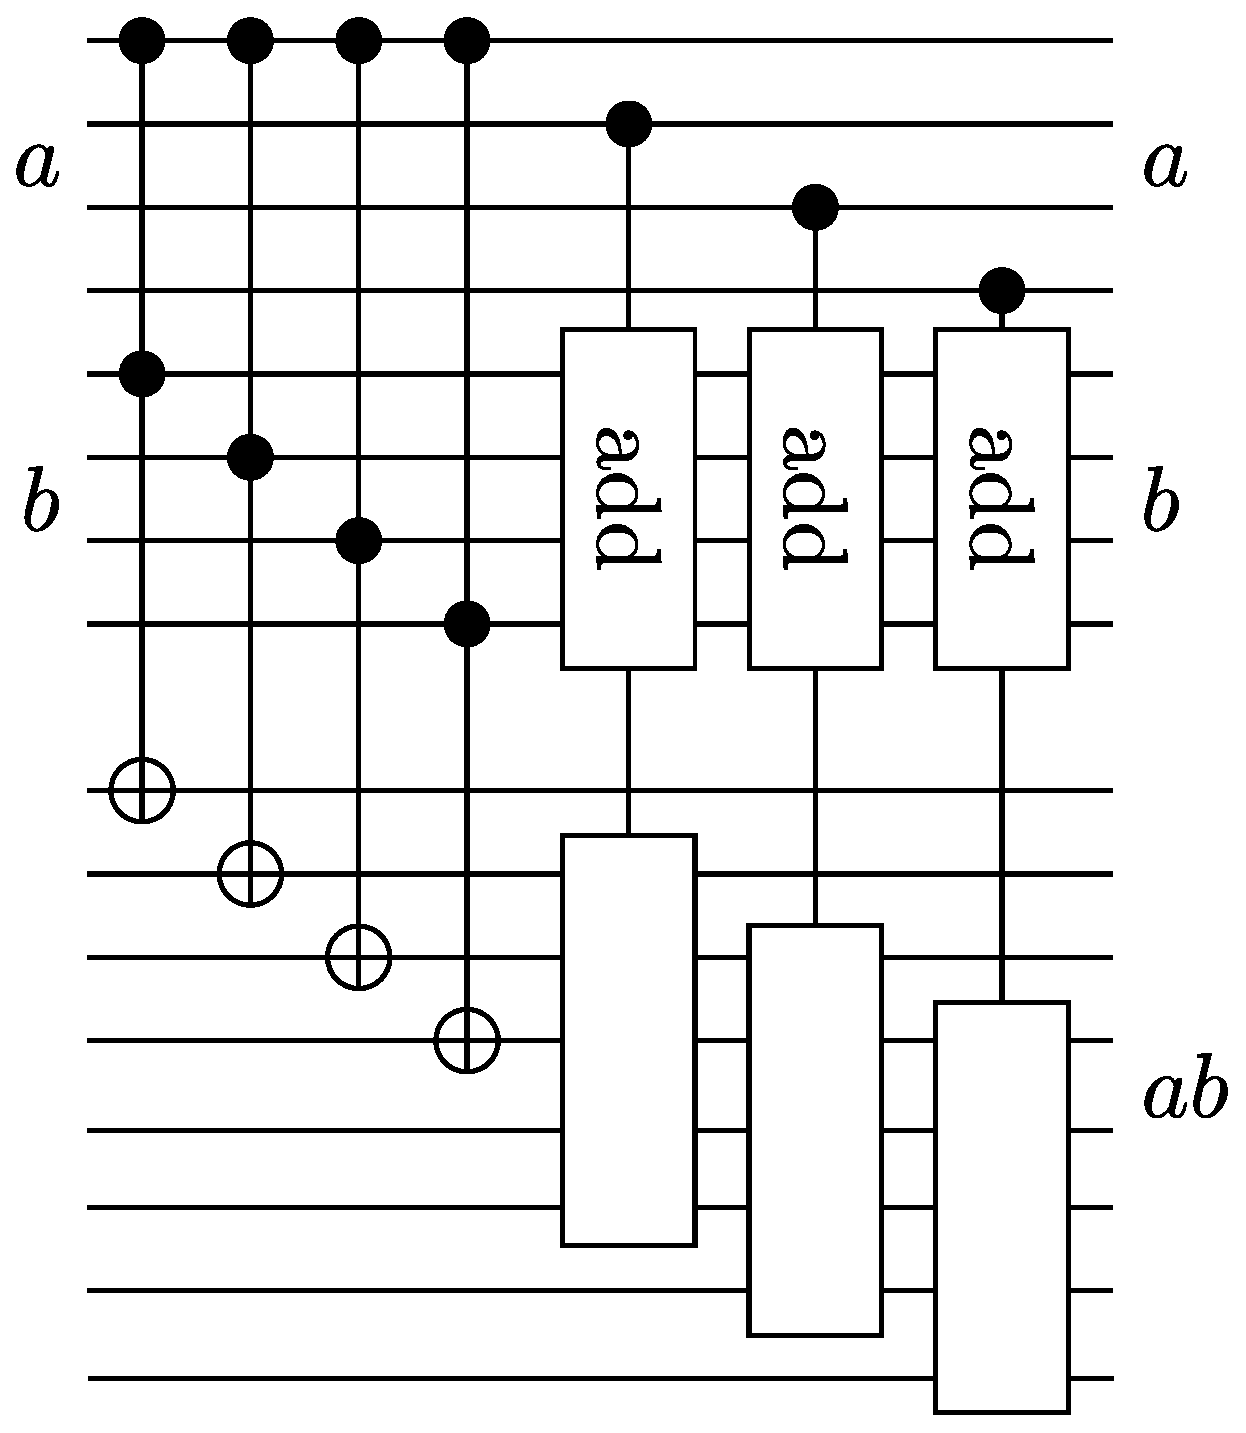
\includegraphics[width=\linewidth]{diagrams/multCtrlAdd}
      \end{figure}
    \end{column}
  \end{columns}
\end{frame}

\begin{frame}
  \frametitle{Karatsuba}
  \begin{columns}
    \begin{column}{5cm}
      \begin{itemize}
        \item Asymptotically lower T-count and lower depth then naive method 
        \item Bad asymptotic bounds for recursive cleanup
        \item More space needed with lazy cleanup 
      \end{itemize}
    \end{column}
    \begin{column}{5cm}
      \begin{figure} 
        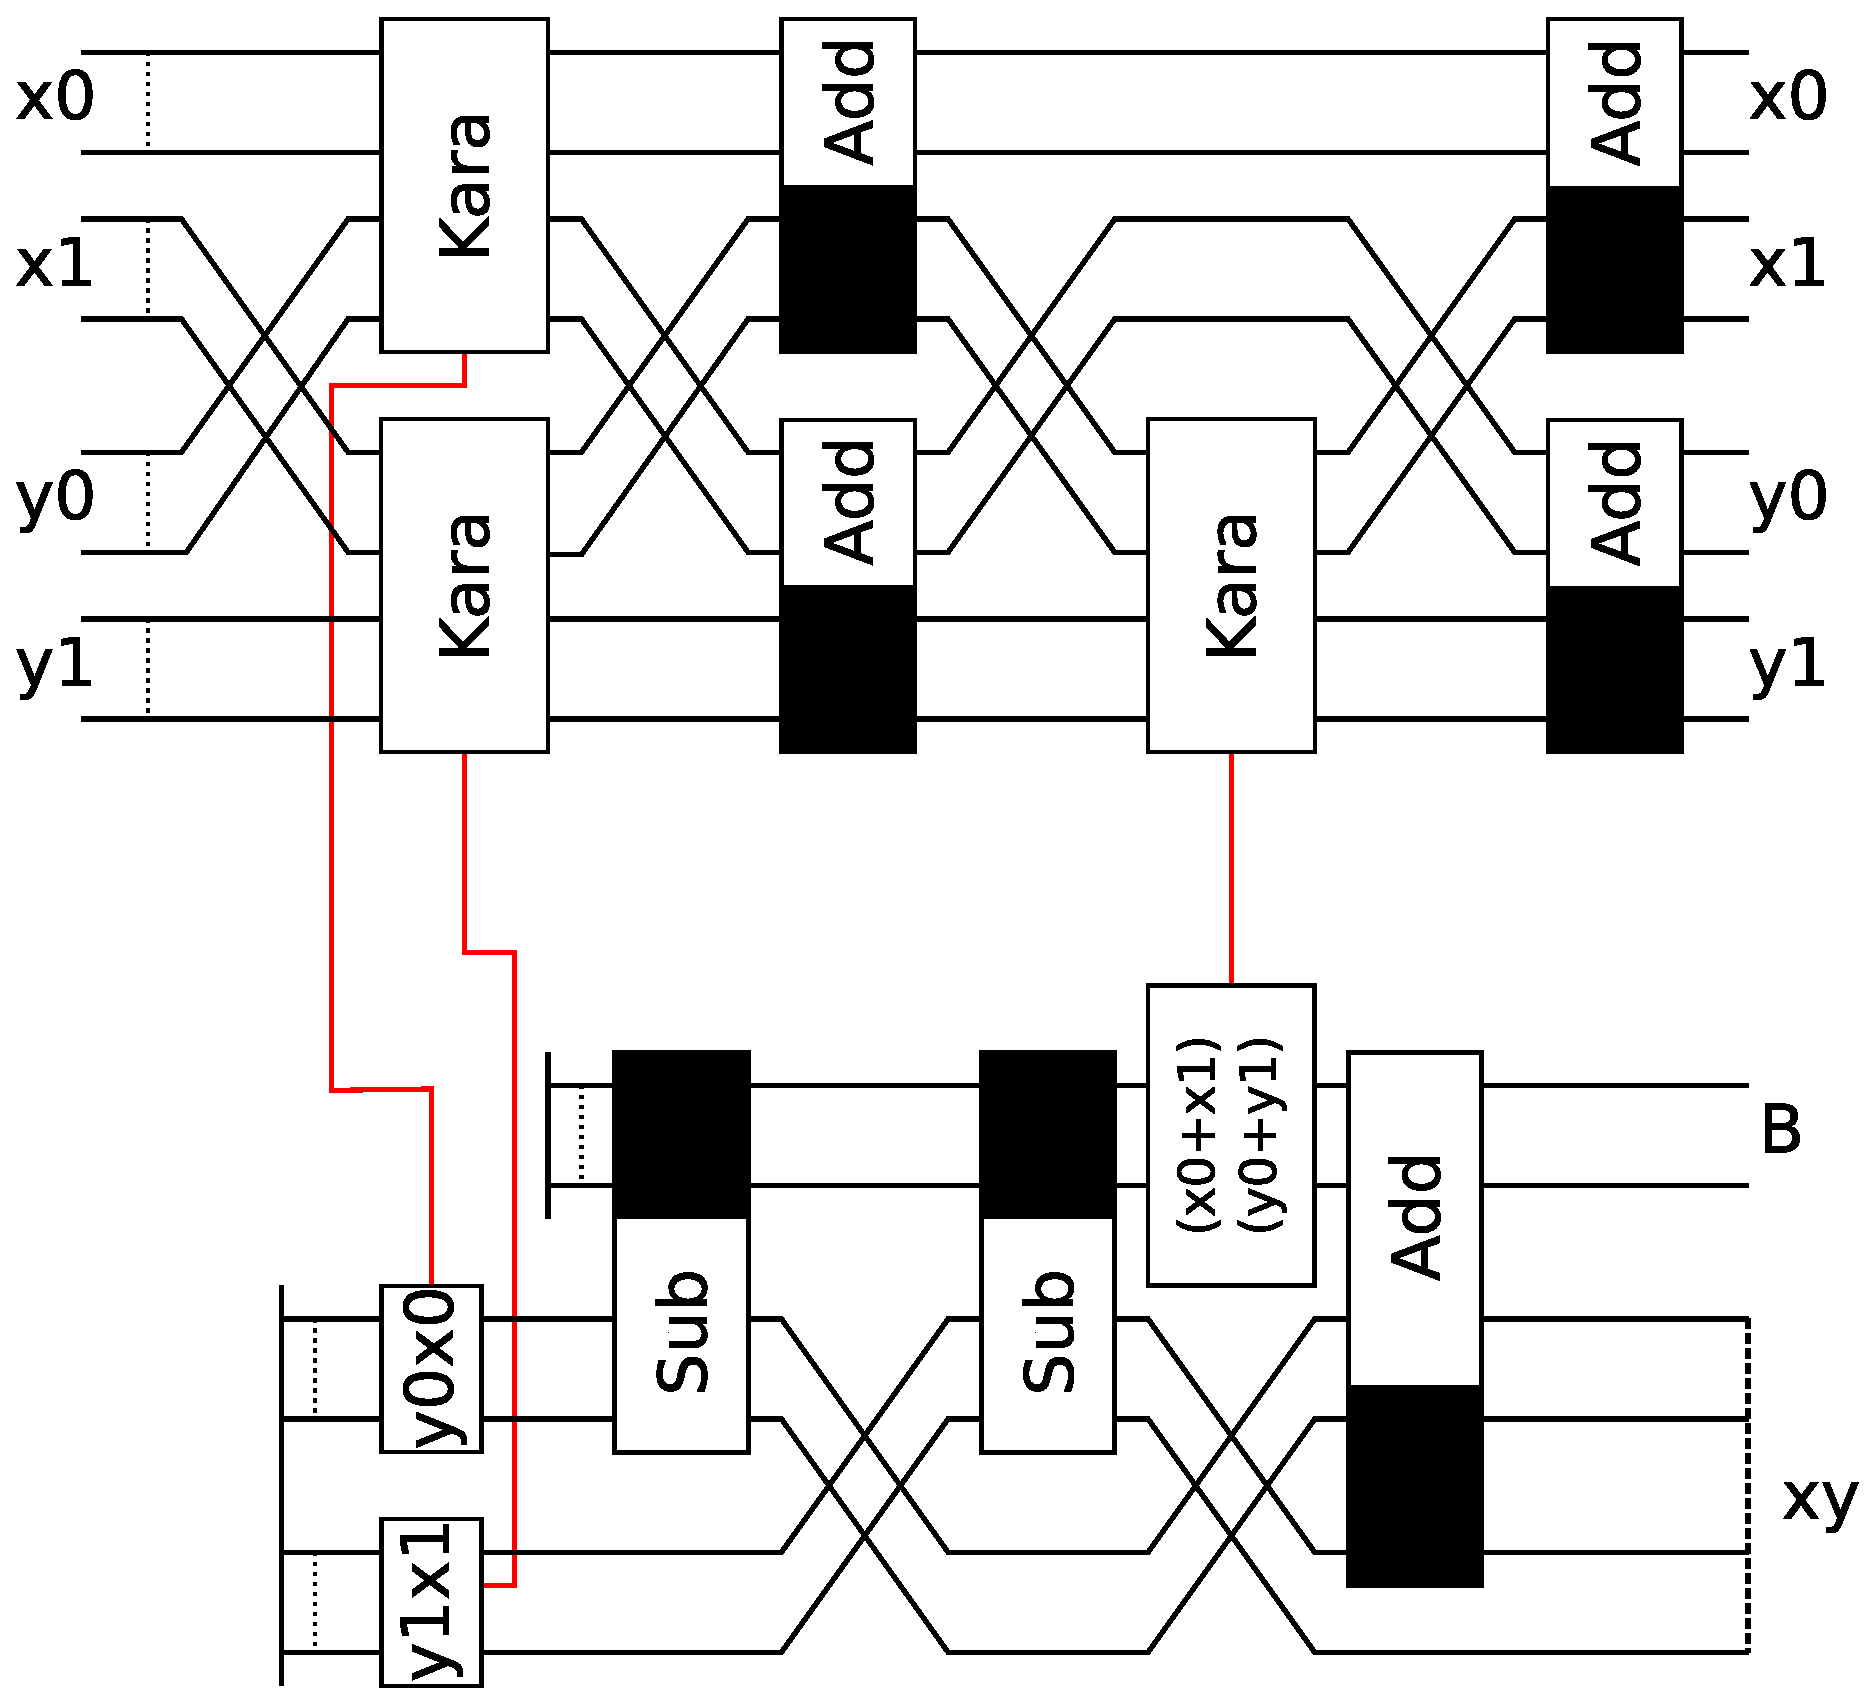
\includegraphics[width=\linewidth]{diagrams/kara}
      \end{figure}
    \end{column}
  \end{columns}
\end{frame}

\begin{frame}
  \frametitle{Karatsuba: Choosing a Cuttoff}
  \begin{figure} 
    \includegraphics[width=\linewidth]{diagrams/karaCutt}
  \end{figure}
\end{frame}

\begin{frame}
  \frametitle{Karatsuba: Choosing a Cuttoff}
  \begin{figure} 
    \includegraphics[width=\linewidth]{diagrams/avgSizeCutt}
  \end{figure}
\end{frame}

\begin{frame}
  \frametitle{Karatsuba: Size}
  \begin{figure} 
    \includegraphics[width=\linewidth]{diagrams/karaSize}
  \end{figure}
\end{frame}

\begin{frame}
  \frametitle{Karatsuba: Depth}
  \begin{figure} 
    \includegraphics[width=\linewidth]{diagrams/karaDepth}
  \end{figure}
\end{frame}

\begin{frame}
  \frametitle{Current/Future Work}
  \begin{block}{Expected to be complete by mid August}
    \begin{itemize}
      \item log, sqrt, trig functions 
      \item Implemented using CORDIC
    \end{itemize}
  \end{block}
  \begin{block}{Future}
    \begin{itemize}
      \item Further improvements to modular arithmetic 
      \item Optimizations when an input is known to be constant at compile time
    \end{itemize}
  \end{block}
\end{frame}


\end{document}
